\chapter{Random Graph Generators and Automorphisms}

\section{Random Graph Models}

The field of random graph theory was started with two independent papers in 1959, each defining models for generating and analyzing random graphs.
A \emph{random graph model} is any system of generating graphs with the influence of chance, with various constraints that describe the desired properties of the resulting graphs.
These two papers began a trend in graph theory that allowed theoreticians and algorithm designers to think about efficiency differently, particularly on NP-Hard and NP-Complete graph algorithms.
Rather than concerning themselves with worst case run time, theoreticians began describing and designing algorithms to satisfy ideas of average case running time over the `class of random graphs'.
Random graphs served as a new lens through which theory could pivot away from the worst case, instead handling common and general cases of problems that were either proven to be impossible in the worst case, or suspected to be so. 

In this chapter, we will discuss multiple models of random graph generation, examine the strengths and flaws of each, and propose alternative mechanisms by which graphs can be generated for more theoretical applications and algorithms.

It is important to recognize that there has been an increase in interest in alternative random graph models in the last ten years.
The majority of these papers focus on exponential random graph models, which are centered around the study of network structure with local and global patterns of connection.
For example, the internet (if sites are viewed as vertices and links as edges), has an exponential in-degree distribution (many more people link to cnn.com than gradybward.com).
Another set of random graph models tries to model social networks, which are categorized by cliques (groups of friends), with alternative connections that symbolize non-group friendships.
For either of these models, algorithmic theory is inadequate if it treats all graphs as equally likely, or if it treats all graph instances as equally likely.
Though this section is not focused on these models, it does adapt some of the characteristics and heuristics of this pursuit to a different goal, of establishing a random graph model for testing algorithms over the set of all graphs.

In this pursuit, we will question what we mean when we say `random' graphs, and make explicit the assumptions, aims and valid applications of any one of our models. 

\subsection{The Erd\"os-R\'enyi Model(s)}

In their seminal paper on random graph theory, Paul Erd\"os and Alfred R\'enyi proposed two different models for random graph generation.
The first of these models will be outlined in this section, and will be referred to as the Erd\"os-R\'enyi Model.
The second was laid out in the same 1959 paper, but was also discovered by an independent contemporaneous mathematician, Edgar Gilbert.
For the sake of clarity, we will refer to the contemporaneously described model as the Gilbert Model, and the one that is about to be outlined as the Erd\"os-R\'enyi Model.

The model $G(N, M$) is defined as choosing a graph G with uniform probability from the set of all graph instances with $N$ edges and $M$ vertices.
The size of this set is $\binom{E_{max}}{M}$, where $E_{max} = \frac{1}{2}(N^2 - N)$ represents the maximum number of vertices possible in a graph over $N$ vertices.
Though the probability of getting any graph \emph{instance} with $N$ and $M$ edges out of this model is uniform, the probability of getting any graph with those constraints is not.
Since the number of representations of a graph fluctuates along with other properties of the graph, this random generator has the flaw that certain graphs are more heavily weighted than others.
This is a flaw that we will discuss at length in discussion of the Gilbert Model.

In the study of random graphs, the Erd\"os-R\'enyi model has not been as popular as the Gilbert model because it is more cumbersome to deal with, and has fewer concrete applications.
Though some papers have utilized this model, the majority of theory is better suited to the combinatorial and probabilistic methods that are made useful by the Gilbert model.
Though knowing the number of edges in a graph gives us some information about the graph, it turns out that the probability of a given edge, and the guarantee of its independence, is significantly more malleable to theoretic goals.

\subsection{The Gilbert Model}

The second model, which we will call the Gilbert model, comes from the mathematician Edgar Gilbert (as well as Erd\"os and R\'enyi) and is denoted $G(n, p)$.
In the Gilbert model, $n$ specifies $N$, the number of vertices in the graph, and every pair of vertices is connected by an edge with a fixed and independent probability $p$.
The Gilbert model is both intuitively pleasing, justified by real world use, and has convenient properties for proof.

The Gilbert Model is an effective model for real world applications where graphs are thought of as occurring naturally without oversight or intervention.
If we think about the configuration of the a network generated by actors acting randomly, the Gilbert model is appropriate.
For example, consider a cocktail party among strangers, where the odds that any two people have a conversation in a given evening are likely independent and uniform.
Or, consider the reproduction of coral, where fertilization of one coral by another is reasonably random through the fluid dynamics that carry, combine and disseminate their pollen.
Gilbert's model gives us the language to describe graphs that pop up in wide-ranging uses, and a model to express the assumptions we frequently make about graphs in practical applications.

Additionally, the Gilbert Model allows us to make bold proof-based claims about random graphs through established combinatorial and probabilistic methods.
For example, if we try to estimate the number of edges within the a Gilbert graph, we simply are asking the binomial question with $n$ and $p$, and we have a readily available probability distribution to answer our questions.
A more interesting example arises when we ask about the number of triangles expected in a large graph.
If our graph is sufficiently large enough, the existence of one triangle does not impact the potential existence of another.
We can express the number of triangles as a simple combinatorial problem: multiply the total number of triangles possible $\binom{N}{3}$ by the probability of all three edges existing $(p^3)$.
This shows how combinatorics gives us tools to deal with Gilbert random graphs, and to make theoretical statements about expectations of the properties of these graphs.

Finally, the Gilbert model has a revelatory connection to matrix representation.
Consider the model with a fixed probability of $p=0.5$ and some fixed $N$.
We will show that this random generator has a uniform probability of selecting any matrix from the set of all valid graph instances of size $N$.

Consider the range of integers $[0, K^2 - 1]$.
If we assume numbers are left-padded with infinite zeros, the $b$th bit of a randomly selected integer from this range has an equal probability of being a 1 or a 0, as exactly half of these numbers have each bit set.
This is trivially true through the fact that there are $K^2$ integers in this range, and $K^2$ different bit strings.
Since each bit string is only achievable with exact probability $(0.5)^K$, each integer is generated with the same, uniform probability.
We will reshape the bit-string into representing each one of the edge variables, and we let $K = E_{max} = \frac{1}{2}(V^2 - V)$.
This establishes a connection between the Gilbert model and a randomly selected matrix from the set of matrices which represent our definition of valid graphs. 
This connection is intuitively pleasing, but further investigation should also show that its implies skewed results for some algorithms which rely on it.

\subsection{Isomorphism Under the Gilbert Model}

One of the first places that theoreticians turned their attention toward after the start of the study of random graphs was the problem of Graph Isomorphism.
The dominant lens of that study was the discussion of naming a class of graphs, and having the following proof structure:
\begin{itemize}
\item{The class of graphs is closed under isomorphism (i.e. all graph instances are in the class of graphs)}
\item{The class of graphs includes a large proportion of all graph \emph{instances}}
\item{Any two graph instances in the class of graphs can be determined isomorphic or not in polynomial time}
\end{itemize}
This approach was undertaken by a large number of theoreticians in the 1960s and 1970s.
A secondary component of these papers became the discussion of alternative algorithms which could solve the cases that were not solved for by the large model of the paper.
It seemed (to paraphrase from Erdos), that graph theoreticians were going to chip away at the problem of graph isomorphism until there was nothing left to chip away.
Yet, as it went forward, the increasingly restricted set of graphs for which no fast algorithm was known did not vanish.
Instead, theoreticians (pardon the projection) were surprised to find that Graph Isomorphism was a hydra that they couldn't vanquish through these means.
No matter the number of large classes of graphs they covered, no matter the diminishing proportion of graphs that were left uncovered, they couldn't find a way to solve all cases.

Hindsight is clear, and we can see that the theoreticians' realization was really a self-reflexive commentary on the work that we are going to be doing in this section.
What they had discovered is that the easy cases in isomorphism are exponentially (in fact, factorially) more common under a Gilbert model than they are if we treat them as algebraic objects.
Thus, even as they shrunk the probability of seeing one of these highly automorphic graphs under a gilbert model, they did little to increase the overall number of graphs that their algorithms covered.

The work we are going to do in this report is taking the opposite approach.
Rather than trying to create algorithms that only cover a set of easy to handle graphs, we are going to ask how we can explicitly look for the harder cases.
There are a number of justifications for this kind of work, but one simple one is the evaluation and clarification of random graph models.
Initial attempts at modeling social networks, first through gilbert models, then through exponential models, failed to appropriately assess the true nature of the problem.
Similarly, algorithm designers who use a gilbert model to test against the `average' graph should have their algorithms checked against a truly `average' graph.

Treating graph instances as graphs allows theoreticians to use easier math, and allows algorithm designers to inflate their claims.
In the next section, we will show how a simple problem (like graph isomorphism) has dramatically different theoretical and experimental analysis when performed over all graphs than when it is performed over all graph instances.

%----------------------------------------------------------------------------------

\section{Disconnect from Graphs as Algebraic Objects}

Though it is the foundation for most probabilistic random graph theory, the Gilbert model is has a different meaning than we typically think when discussing `random' generators of other kinds.
When we consider most other discussions of `uniform randomness', we state the assumption that the result element was selected from its set with a uniform probability.
Moreover, we generally assume that each object within that pool was represented the same number of times.
When I say `a randomly generated integer from the range', we are all agreeing on assumptions of what integers fall within this range, as well as how many times each is in our pool for selection (namely, once). 
Whereas, when I say `a randomly selected word from a book', there is the possibility that common words are more likely to occur, or it could mean that I found the unique set of words in the book, and I am selecting from that.

This is where random graph theory and colloquial understandings of randomness miss one another.
Throughout this work I have gone to great lengths to distinguish between graphs (an entity that has a given structure), and graph instances (a given representation of that structure).
Most graphs have many distinct graph instances; many different ways of representing themselves, but this number varies as a function of the properties of the graph.

The problem with the two models outlined above is that they select a random \emph{graph instance} with a uniform probability, but this does not translate to our understanding of graphs as algebraic objects, which denote structure irrespective of representation.
Thus, a model which chooses graph instances with uniform probability does not choose graphs with uniform probability, just as selecting a word at random off of the page of a book is not equivalent to selecting a word from all of the words in the book with uniform probability.

Consider an illustrative example with two graphs, G and H, on $N$ vertices and $M$ edges.
Graph G has only the trivial automorphism, and Graph H has an automorphism group with 20 elements.
It is well established that the number of distinct matrix representations (and thus distinct labelings) of a graph is equal to $\frac{N!}{|Aut(G)|}$.
Thus, the number of graph instances that represent graph G is $N!$, while the number of graph instances that represent graph H is $\frac{N!}{20}$.
Since graph instances are really just a way about talking about the number of matrices which represent the graph, this means that in the set of all valid undirected, non-looped graph matrices, there are 20 times as many which represent G as represent H.
This is critical because the two models of selecting random graphs select a matrix with a certain number of ones (some number of edges) with equal probability.
Even when the probability is not $p=0.5$ as it was in the illustrated case, it is clear that this is true.
This means that the probability of selecting a matrix which represents graph G is twenty times more likely than selecting a matrix which represents graph H under either `random' graph generator.

Though this seems like a semantic difference, as I will show over the next several sections, it has critical implications for the algorithms that use it to argue about computational complexity.

\subsection{Comparing the Distribution of Graph Connectivity}

In Chapter 1, we described the overall distribution of graphs as algebraic objects with respect to their connectivity.
We can also model the connectivity if we are considering the set of graph instances.
Since there is a one to one correspondence between graph instances and the set of all valid zero-diagonaled, binary symmetric matrices, we can discuss the connectivity of graph instances as a function of the binomial distribution.
That is because we can view the process of random graph instance generation under the gilbert model with probability .5 as a sequence of disjoint (as equally probable) binary variables, one per edge.
Thus the number of edges in a Gilbert random graph follows a binomial distribution with $E_{max}$ trials and fixed probability of success $\frac{1}{2}$.

The variance of such a model is known to be 
$$Var(Binom(n, p)) = (1-p) * p * n = E_{max} * .5 * .5 = \frac{E_{max}}{4}$$
Since we want to normalize our distribution so that the x values represent connectivity, we divide by the number of edges possible (after we convert to the standard deviation by taking the square root:
$$\sigma_{norm}(|E(G_{inst})|) = \frac{\sqrt{Var(Binom(E_{max}, .5))}}{E_{max}} = \frac{\sqrt{1/4 * E_{max}}}{E_{max}}  = \frac{1}{2\sqrt{E_{max}}}$$
Using these values, we can plot the relative sigmas for the distribution of graphs relative to their connectivity for both of the sets: the set of all graph instances, and the set of all graphs as algebraic objects.
Doing this we get the graph shown in figure \ref{fig:sigmaconvergence}.

\begin{figure}[h]
\caption{\emph{Sigma of Connectivity Distribution for the Set of Random Graphs and the Set of Random Graph Instances}}
\centering
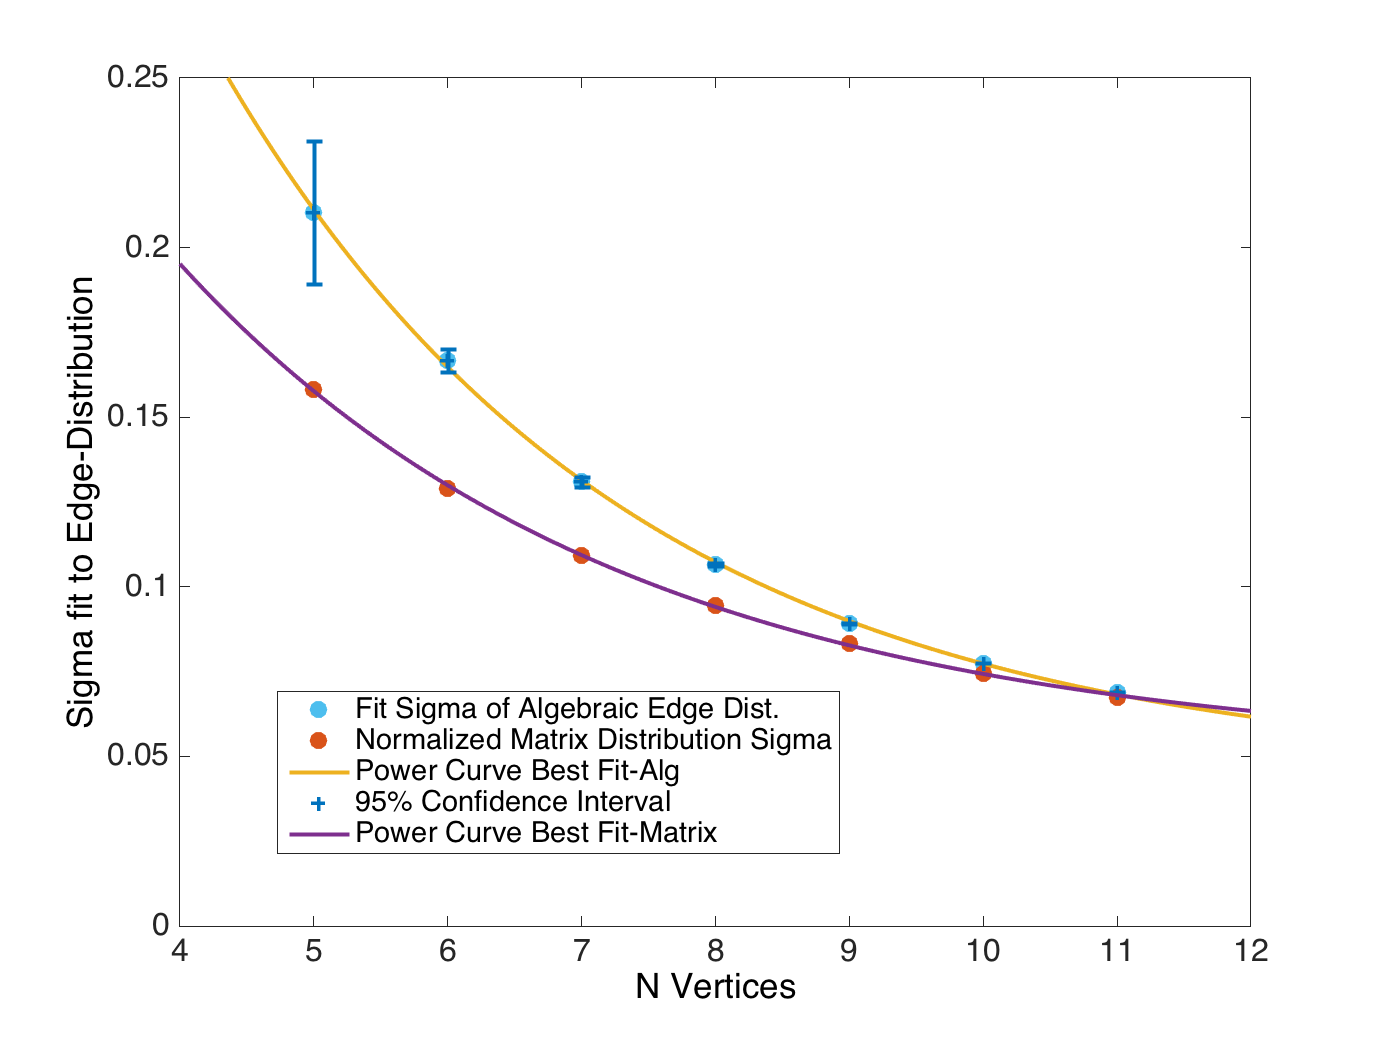
\includegraphics[width=\textwidth]{decreasingsigmawithbinom}
\label{fig:sigmaconvergence}
\end{figure}

Note that the values appear to shrink in their disparity, a remarkable observation, which gives us an idea of how the two sets/distributions differ with respect to the number of edges they produce as a function of $N$.
However, fitting exponential functions to each muddles the question: are they converging or intersecting and diverging again?
Note that even a convergence doesn't tell us about other properties of the sets of graphs.
Similarity in the distribution of the number of edges (or connectivity) does not equate distributional symmetry.
However, what we can see is that the Gilbert graph generator models the number of edges successfully for values of $N \approx 11$, and for larger values it may or may not  mirror this distribution.

%----------------------------------------------------------------------------------

\section{Specifically Disadvantaging Highly Automorphic Graphs}

Dominant models of random graph generation specifically preference graphs with fewer non-trivial automorphisms over graphs that have many automorphisms. 
This flaw is most glaring when discussing average or worst case running time over the `random' class of graphs.
Many algorithms make exciting claims about their performance on `random' graphs, but
we will show how theoretical and practical analysis of performance changes dramatically under different random graph generators.

\subsection{Two Quick Justifications}

To get an initial sense of this problem, we will first examine the relative probabilities of selecting a Co-Cycles graph from the set of graphs of size 10.
Since we know all 116 Co-Cycles graphs over 10 vertices, we can (without much computational effort) calculate the relative probabilities of generating a Co-Cycles graph under the standard (Gilbert) model and under the idealized model.
The results are not shocking, but a notable difference is apparent:
$$P(CoCycles(G) | G \in Gilbert) = \frac{\sum_{g \in CoCycles}^{116}M_{reps}(g)}{N Matrices} = \frac{260820000}{3.5184 \times 10^{13}} = 7.4130 \times 10^{-6}$$
$$P(CoCycles(G) | G \in Gilbert) = \frac{N CoCycles Graphs}{N Graphs} = \frac{116}{12005168} = 9.6625 \times 10^{-6}$$

Though these are not exorbitent differences, it should be noted that there is a difference of 23\%, meaning that by using a Gilbert random graph generator, you are 23\% less likely to observe a co-cycles graph as a result of generating one random graph than you would be via an idealized generator.
In this case, the difference between the generators is clearly appreciable, but not severely limiting.

As a second example, we will compare the most and least likely graphs to be observed under either random graph model.
In an idealized random graph generator, all graphs have equal probability of being selected.
Thus, the ratio of the most likely to least likely is exactly 1.

In a Gilbert random graph generator (abstracting over p, as discussed earlier), graphs that are fully automorphic (where the automorphism set contains all one-to-one mappings), are the least likely to occur.
One such graph is the fully connected graph, or the complete graph ($K_N$).
This is simply because the number of matrices which represent them is given by $M_{reps}$, and the probability of selecting a the complete graph is thus:
$$P(G = K_N | G \in Gilbert) =  \frac{M_{reps}(K_N)}{NMatrices} = \frac{N! / |Aut(K_N)|}{2^{.5N(N-1)}} = \frac{N! / N!}{2^{.5N(N-1)}} = \frac{1}{2^{.5N(N-1)}}$$
However, if we examine a graph with only the trivial automorphism ($G_{TA}$):
$$P(G = G_{TA} | G \in Gilbert) =  \frac{M_{reps}(G_{TA})}{NMatrices} = \frac{N! / |Aut(G_{TA})|}{2^{.5N(N-1)}} = \frac{N! / 1}{2^{.5N(N-1)}} = \frac{N!}{2^{.5N(N-1)}}$$
Thus, the ratio of these probabilities is always going to be $N!$.

These two examples give us a really important message: the difference between the Gilbert and Ideal models is frequently substantive, but its effects can be mild (as in the case of co-cycles graphs), or extreme (as in the case of selecting a perfectly automorphic graph).
What largely determines the degree of this distortion is the \emph{average number of automorphisms in the set that is being examined}. 
The larger this number, the more distortionary the Gilbert Model is when compared to the Idealized model.

\subsection{Theoretical Average Case Comparison}

Consider a standard canonical labeling algorithm.
This algorithm has two abstract components, one which correctly places vertexes into Similar Vertex Sets (SVS), and another which finds a canonical labeling given an accurate SVS partition.
If we take the first part of this algorithm as given, and assume that it can be computed in polynomial time (a reasonable assumption, as discussed in the section on SVS), then the running time of the algorithm is contingent upon the number of matrices we need to evaluate against some canonical property.
One common property for canonization is selecting the adjacency matrix which is the lexicographically smallest (or largest) representation of the graph.
It is reasonable to assume that the second half of the algorithm dominates the running time of the overall algorithm, as it is the piece that is inherently exponential based on the number of representations of the matrix.
Thus,  we can express the running time of the overall algorithm in terms of $O(|Aut(G)|)$, as this is the number of possible labelings we will have to examine to find our canonical one.

The selection of this simplified algorithm for analysis is not an accident: we have chosen it because the number of matrix representations ($M_{rep}(G)$) for a given graph $G$ is $\frac{N!}{|Aut(G)|}$.
Thus, if we are considering the average running time of this canonization algorithm ($\xoverline{T}_{Gilbert}$) over the set of all graph instances ($G_{inst} = G(A)$ for $A \in \{\{0,1\}^{N \times N}\}$) (i.e. using the standard models for random graph generation), we come to different conclusions if we consider the set of possible graphs $G_{inst}$, versus if we consider the set of all graphs as algebraic structural objects ($G_{alg}$).
$$\xoverline{T}_{Gilbert} = \frac{ \sum_{g \in G_{inst}} O(T(g))}{|G_{inst}|}$$
$$\xoverline{T}_{Gilbert} = \frac{ \sum_{g \in G_{alg}} O(T(g)) * M_{reps}(g)}{|G_{inst}|}$$
$$\xoverline{T}_{Gilbert} = \frac{ \sum_{g \in G_{alg}}  |Aut(g)| * \frac{N!}{|Aut(g)|}}{|G_{inst}|}$$
$$\xoverline{T}_{Gilbert} = \frac{ \sum_{g \in G_{alg}}  N!}{2^{.5(N^2 - N)}}$$
$$\xoverline{T}_{Gilbert} = \frac{ |G_{alg}| * N!}{2^{.5(N^2 - N)}}$$

This property might not look like it tells us much, but we can actually approximate what it looks like for different values of $N$, since we have the frist nineteen values of this sequence from OEIS sequence A000088.
This data is shown below.

However, if we attempted to select a graph from the set of all graphs of that size, we would find that: 
$$\xoverline{T}_{Ideal} = \frac{ \sum_{g \in G_{alg}}  O(T(g)) }{|G_{alg}|}$$
$$\xoverline{T}_{Ideal} = \frac{ \sum_{g \in G_{alg}}  |Aut(g)|}{|G_{alg}|}$$
$$\xoverline{T}_{Ideal} = \text{Average Number of Automorphisms over Graphs}$$

Some sample numbers to give you the scale of these disparities is given below.

The takeaway here is that specifically disadvantaging a class of graphs (namely highly automorphic graphs) warps our analysis of running time in a substantive way, not only for fringe algorithms, but for well studied algorithms too.
We can show this through the theoretical proof as shown above, but we can also show it through data describing actual algorithm performance.

\subsection{Practical Average Case Comparison}

The NAUTY package is one of the quickest algorithms for canonical labeling.
Though its performance is weaker on some graphs (like the Miyazaki, for example), in general, its canonical labeling algorithm is widely regarded and frequently used.

I ran the NAUTY canonization algorithm on batches of graphs with different numbers of edges, to get a sense for how the running time changes when we change the way that we randomly generate the graphs.
Shown in figure \ref{fig:nautyperformance10} is how the NAUTY algorithm performs against varrying values of $p$ for $N=10$.
Each was run thirty times, and the margin of error (as a 95\% Confidence Interval) is shown around each of the estimates.

\begin{figure}[h]
\caption{}
\centering
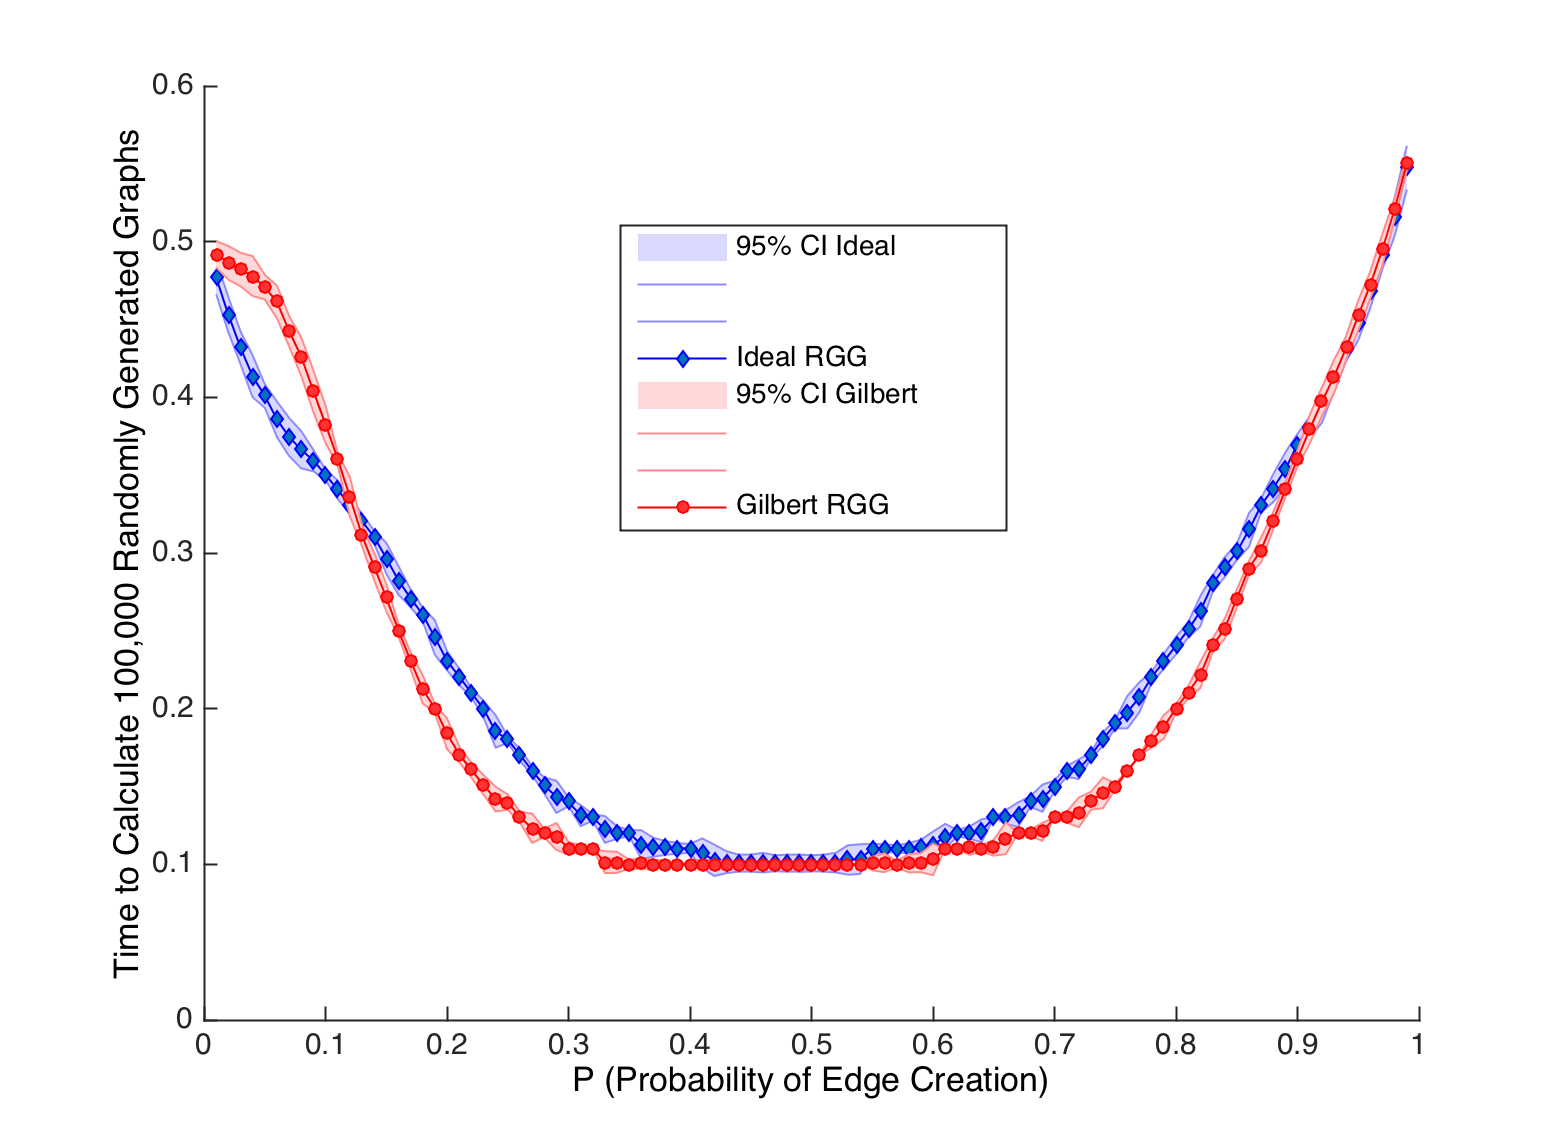
\includegraphics[width=\textwidth]{nautyperformance}
\label{fig:nautyperformance10}
\end{figure}

We can see from this figures that not only does NAUTY have slower performance on `Idealized' random graphs, but there are crossover effects.
The integral between these curves works out to about a 10\% increase in running time between the Gilbert RGG and Idealized RGG.

Both in theory and in practice, distinguishing between 'random graph' and `random graph instance' has significant implications.
It is very possible that misuse of the Gilbert model has understated the true average and worst case time complexity for a number of algorithms, including the NAUTY algorithm.

\subsection{Should We Never Use the Gilbert Model?}

The short answer to this question is no, the Gilbert model is remains relevant (even dominant) even when we embrace these flaws.
The primary argument for the Gilbert model is not its application to questions of theory, \emph{but questions of practice and natural occurrence}.
Most applications of graph theory to world problems are based around structures that are naturally arising, without centralized planing or design.
It is much more likely that some graph that is found in the world will be non-automorphic than have some kind of inherent and difficult to describe complexity.
This is because if we look at graph building as a process (in the Gilbert model), or as a probabilistic construction (in the Erdos-Reyni model), then some outcomes are more likely than others.
This is well in line with the assumptions of the models: that graph instances are suitable placeholders for their graphs.

Rather, what we have been criticizing is the \emph{application} of the Gilbert model to questions about theoretical algorithmic complexity.
In graph theory, we hold a meaningful distinction between graphs and graph instances, a distinction only made at the theoretical level.
It is thus inappropriate to use a model which ignores this distinction, and ignores it in such a way as to specifically disadvantage certain classes of graphs.
This allows theoretical arguments about graph algorithms to underweight what we consider `hard' cases, and overweight what we would generally consider `easy' cases.

This distinction is important.
In practice, graphs that arise in the world are likely to be selected randomly from the set of graph instances.
However, in graph theory, where we consider isomorphic graph instances to be fundamentally equivalent, the assumptions of the Gilbert model are antithetical to other assumptions of graph theoretic research.

\section{Measuring and Comparing Random Graph Models}

Our mandate suddenly becomes: `well, what can we do which is better?'
Establishing an intuition to answer this question requires us first to understand what we would think of as `ideal', and see if we can approach that model.

\subsection{An Ideal Random Graph Model}
To allow our comparisons to be explicit, we will use the same nomenclature to describe an idealized generator as we do with the Gilbert model, so that they are directly comparable.
Thus, our ideal random graph model will take two input parameters, $N$ and $p$, where $p$ describes the probability of getting any given edge existing.
Note that this explicitly breaks from the idea of edge independence that is assumed in the Gilbert model.
Rather, we are assuming that the probability of any given edge existing is $p$ if we have no knowledge about the rest of the graph.
We will define our `Ideal' generator as one which first selects a number of edges $M$ from the binomial distribution with $E_{Max}$ trials and trial success probability $p$.
After selecting $M$ as an observation from this random distribution, we will select a graph from the set of all graphs of $N$ vertices and $M$ edges with uniform probability.
To accomplish this task, we will enumerate all graphs of that size, and select from that fully defined set.

The flaw in this scheme is obvious.
Our `Ideal' generator is only possible by this methodology so long as you can enumerate all graphs of a given size.
There are 24637809253125004524383007491432768 non-isomorphic graphs over 19 vertices, so this is not remotely sustainable methodology for a random generator.
If we cannot rely on an ideal graph generator, are we doomed to stick with the Gilbert model?
Or, could we create a model that is better than the Gilbert model (closer to our ideal), while being computationally reasonable?

\subsection{An Equivalent Ideal Random Graph Model}

Another way to view our equivalent random graph model is as a overlaid construction on top of a standard, Gilbert, random graph model.
Since we know that the Gilbert random graph model produces a graph with a probability proportional to its number of automorphisms, we can actually create a random graph generator which is equivalent to our idealized model by systematically throwing out graphs with probability inverse to their probability of showing up.
The algorithm which generates to this model is not guaranteed to halt, but does simulate our idealized random graph generator, even over large values of $N$.

\begin{lstlisting}[frame=single]
while true:
	g = gilbertRandomGraph(N, p)
	na = |Aut(g)|
	p = Math.rand(0, 1)
	if (p < (na / N!))
		return g
\end{lstlisting}

Here we find a gilbert random graph, and calculate the number of automorphisms that it has.
That gives us knowledge of how many times we would expect it to occur in a sample of $2^{E_{max}}$ random graph instances, namely $N! / na$ times.
Thus, we weight any randomly observed random graph instance by the inverse of this value.
This equalizes the probability of getting any graph, regardless of its number of automorphisms.

This methodology is, unfortunately, equally unsustainable.
This is an example of a geometric process, where we will have to go a certain number of trials before finding a success and stopping. 
The probability of a success on any given trial is $p = \frac{|G_{alg}|}{|G_{inst}|}$, which approximates the $p = fact^{-1}(N) = \frac{1}{N!}$ growth function.
Thus, for even a small number of vertices, the expected number of trials that need to be generated before a success is found is very large, as it is given by $1/p = N!$. 
For example, if $N=10$, we would expect to have to examine 3.6 million graphs before finding one which is returned successfully.

This too, is not a sustainable methodology for random graph generation.

\subsection{Establishing a Methodology for Random Graph Generator Evaluation}

So what can we do that is better?
Answering that question required some really deliberate thought.
I knew lots about what I didn't want to do:
\begin{itemize}
\item{I didn't want to use subjective measures to support one random graph generator over another.}
\item{I didn't want to write generators and then use collected data to support them.}
\item{I didn't want to focus in on singular ways of looking at the quality of the graphs that I generated.}
\item{I didn't want to allow my own intellect and lack of creativity be a limiting step on the way to a better generator.}
The process that I decided on attempted to address all of these concerns, and was designed to avoid the pitfalls of bad computer science: overfitting, statistic selection, and rigidity.
\end{itemize}

I decided on a wide portfolio of statistics each of which is calculated over a sets of graphs.
These statistics are inherently heuristic, but each attempts to capture some property of the graphs that are generated, or some property of how the set looks as a whole.
Each of the statistics I decided on is meant to describe some property of a set of graphs, but it does not establish an `idealized' or theoretical value for that statistic.
Though for several of these metrics we know how to express the ideal/expected probability, that is not always the case (or not always known to be the case0.
These metrics serve as a way for us to identify and name ways that random graph generators fail us, and challenge us to do better, to compare a proposed solution to an ideal or standard solution in quantifiable and concrete terms.

The set metrics is described in the next section, and they vary in computational complexity and broad descriptiveness.
I set up a (pardon the brag) BEAUTIFUL system for calculating these statistics over arbitrary datasets.
I created an idealized random generator (as described above), and a Gilbert random generator, and verified the accuracy of the results produced through this computational system over the initial results from each.

Most importantly, I set up these metrics, this system, and the baseline Gilbert/Ideal metric values before I wrote a line of code which randomly generated graphs.
This is really important to me, because it frees the results of this work from the publication and statistic selection bias that plagues research everywhere.

\subsection{Graph Set Metrics}
Below are the metrics that I compared across graph sets generated by different random graph generation procedures.
Though I calculated some more statistics for personal use and discovery, the ones included below are the `single result' statistics.
Others were distributional properties that were not easily captured and compared (except through distributional goodness of fit tests, which only give us an idea of alikeness, not of directed difference).
The reliance on singular metrics as a means of comparison allows us to evaluate systems of random graph generation automatically, and come up with similarity tests that are divorced from our intuition and hypotheses.

Described below are each of the metrics that are calculated over every set of random graphs that were generated.
Each is labeled a statistic (implying a singular value used to judge the generator) or a distribution (connoting that it was not used in the systematized evaluation of generators).
Each is listed under its acronym, which can be found throughout my code and tests. 

\subsection{Graph Set Metric Reference, Coding and Description}

\begin{itemize}

\item{ADIAM - Set Statistic - Average Graph Diameter - Take the diameter of each graph, and average over all graphs in the set}
\item{ADSM - Set Statistic - Average Degree Sequence Mean - take the mean of degree sequence of each graph, and average that across all graphs}
\item{ADSMD - Set Statistic - Average Degree Sequence Median - take the median of the degree sequence of each graph, then average that across all graphs}
\item{ADSMN - Set Statistic - Average Degree Sequence Minimum - take the degree of the least connected node in each graph, then average that across all graphs}
\item{ADSMX - Set Statistic - Average Degree Sequence Maximum - take the degree of the most connected node in each graph, then average that across all graphs}
\item{ADSR - Set Statistic - Average Degree Sequence Range  (i.e. Find the difference in degree between the most and least connected node, and average over all graphs in the set}
\item{ADSV - Set Statistic - Average Degree Sequence Variance - take the variance of the degree sequence of the graph, then average across all graphs}
\item{ALNA - Set Statistic - Average of the Logarithm of the Number of Automorphisms - Find the number of automorphisms that each graph has within the set, take the logarithm of each, then average across the logged results}
\item{ANA - Set Statistic - Average Number of Automorphisms - find the number of automorphisms for each graph, then average that across the set}
\item{ANCC - Set Statistic - Average Number of Connected Components - take the number of connected components of each graph in the set, then average across all of them}
\item{ANQUAD - Set Statistic - Average Number of Quadrilaterals - The Average number of non-trivial (non-edge repeating) quadrilaterals across all graph instances within the graph set.}
\item{ANR - Set Statistic - Average Number of Repeats - The average graph, when selected from the set in question, will have this expected number of equivalent instances in the set}
\item{ANTRI - Set Statistic - Average Number of Triangles - The Average number of triangles across all graph instances within the graph set.}
\item{CP - Subset - Co-Cycles Graphs - The intersection between the set of all $V=10$ co-cycles graphs and the given set}
\item{DIAMV - Set Statistic - Variance in the Diameter of Graphs - calculate the diameter of each graph, and calculate the variance of the set as a whole}
\item{DSMDV - Set Statistic - Degree Sequence Median Variance - Take the median degree of each graph, and calculate the variance over all graphs in the set}
\item{DSMNV - Set Statistic - Degree Sequence Minimum Variance - Take the minimum degree of each graph, and calculate the variance over all graphs in the set}
\item{DSMV - Set Statistic - Degree Sequence Mean Variance - Take the mean degree of each graph, and calculate the variance over all graphs in the set}
\item{DSMXV - Set Statistic - Degree Sequence Maximum Variance - Take the maximum degree of each graph, and calculate the variance over all graphs in the set}
\item{DSVV - Set Statistic - Degree Sequence Variance Variance - Take the variance of the degree sequence of each graph, and calculate the variance over all graphs in the set}
\item{FC - Set Property - Frequency Count - The number of isomorphic graph instances associated with each one of the graphs in the set}
\item{FFC - Set Distribution Counts - Frequency Count Counts - The counts that correspond to FFVs, the frequency with which graphs show up in our random set}
\item{FFV - Set Distribution Bins - Frequency Count Bins - The discrete values for which there exist graphs in our set that poses that number of instances in the set, this is really just a bin count for FC}
\item{MLNA - Set Statistic - Median of the Logarithm of the Number of Automorphisms - Find the number of automorphisms that each graph has within the set, take the logarithm of each, then find the median across the logged results}
\item{MNR - Set Statistic - Maximum Number of Repeats - The graph in the set that was selected the most times was selected this many times}
\item{NA - Graph Statistic - Number of Automorphisms - Counts the number of automorphisms that a graph has by finding the number of unique matrices that describe a graph}
\item{NAB - Set Distribution Bins - Number of Automorphisms Bins - The unique values of NA, to provide histogram alongside NAC}
\item{NAC - Set Distribution Counts - Number of Automorphisms Counts - The counts of the NAB, as in a histogram}
\item{NCCV - Set Statistic - Variance in the Number of Connected Components - take the number of connected components of each graph in the set, then take the variance of the set}
\item{NCP - Set Statistic - Number of Co-Cycles graphs - Same as Co-cycles graphs, this only applies to graphs of size 10 and larger, counts the number of Co-Cycles graphs (which tend to be highly automorphic) in the overall set of graphs}
\item{NE - Set Statistic - Number of Edges - the average number of edges in the graph set. This should be the same across generators, as we are specifying $p$, and asking for a large sample size}
\item{NR - Set Statistic - Number of Regular Graphs - the number of regular graphs in the graphset}
\item{NUG - Set Statistic - Number of Unique Graphs - The proportion of graphs within the set that are only generated once}
\item{ODSPL - Set Statistic - Overall Degree Sequence Poisson Distribution Lambda  - Find the set of all of the degrees of all of the graph, then fit a poisson distribution to this distribution. Report the lambda that defines this poisson distribution}
\item{PCONN - Set Statistic - Probability of Connectivity - take the number of fully connected graphs, and divide by the total number of graphs in the set}
\item{PDL - Set Statistic - Poisson Distribution Lambda - Take the distribution of the number of times that each graph is represented by an instance within a graph set, and set this distribution fit to a poisson distribution, reporting its lambda}
\item{PQRA - Set Statistic - Percentage Quazi-Regular A - Percentage of graphs where the degree sequence range is less than or equal to 1}
\item{PQRB - Set Statistic - Percentage Quazi-Regular B - Percentage of graphs where the degree sequence range is less than or equal to 2}
\item{PQRC - Set Statistic - Percentage Quazi-Regular C - Percentage of graphs where the degree sequence range is less than or equal to $sqrt(N)$}
\item{PTRIL - Set Statistic - Probability Triangle-less - the Probability that a graph instance selected randomly from the graph set is triangle-less.}
\item{SQNR - Set Statistic - Sum of Squared Number of Repeats - A measure of how dispersed the distribution is, calculated as $FFC \dot (FFV^2) / nGraphs$}
\item{UG - Set Property - Unique Graphs - The canonical form of all of the graph set's graphs, with duplicates removed (if they existed)}
\item{VLNA - Set Statistic - Variance of the Logarithm of the Number of Automorphisms - Find the number of automorphisms that each graph has within the set, take the logarithm of each, then find the variance of the logged results}
\end{itemize}

\subsection{Establishing Baselines for Graph Set Metrics}

Once we set up these metrics, we need to find a way to systematically compare them within our desired context: building a random graph generator which models an idealized random graph generator.
To do this, I established baseline understandings for each one of the metrics, over a problem `domain':
\begin{itemize}
\item{Number of Graphs - I decided to operate over sets of 1000 graphs.  It allowed us to get reasonable numbers for standard deviations and not use an excess of CPU time}
\item{Number of Vertices - I baselined the metrics over graphs of size 4 to size 10.  This allowed us to see what the metrics looked like on an overrepresented graph set, and on a sample set.}
\item{Probability of Edges - I used p from the set $[.1, .2, .3, .4, .5, .6, .7, .8, .9]$. I figured that focusing on sparse, dense or intermediate graphs might introduce biases that I hadn't accounted for, so I decided for the most generic set possible.}
\item{Number of Trials - For each one of these baseline scenarios, I performed 30 trials}
\end{itemize}

Thus, in the end, there were $2 \times 9 \times 7 \times 30 = 2780$ sets of 1000 graphs that were used to create our baseline metrics.

For each one of the statistics we calculated the mean and standard deviation of the sampled metrics over both algorithms.
That resulted in two sample means and sample standard deviations, for the ideal and gilbert graph models: $\xoverline{x_I}, \xoverline{x_G}, s_I$ and $s_G$. 
Using these values, I came up with a simple and intuitive way to measure a new random graph generator, given its value for $\xoverline{x_N}$ and $s_N$ and the number of samples that were used to compute each, $n_N$.
This methodology compares the t values in two tests of significance for two unknown means and unknown standard deviations.
In a test of unequal unknown means and standard deviations, the slightly modified t-statistic is given by:
$$T(A, B) = T(\xoverline{x_A}, \xoverline{x_B}, s_A, s_B, n_A, n_B) = \frac{|\xoverline{x_A} - \xoverline{x_B}|}{\sqrt{(s_A^2 / n_A + s_B^2 / n_B}} $$
And our scoring mechanism for a metric and generator is given by:
$$ \text{Score for Metric M} = -1 * \text{min} \bigg[ \ln \Big( \frac{T_M(I, N)}{T_M(I, G)} + e^{-10} \Big), 10 \bigg] $$
Lets break down this scoring mechanism:
\begin{itemize}
\item{First off, $T_M(A, B)$ is strictly greater than or equal to zero (and all of our metrics have non-zero $T_M(I, G)$ values), thus the fraction in the logarithm is defined and in the range $[0, \infty)$. When we add $e^{-10}$, we shift that range up to $[e^{-10}, \infty)$, meaning that the logarithm's value will be bounded between $[-10, \infty)$ }
\item{Next, we take the minimum of this score and 10, to bound the individual score between $[-10, 10]$.}
\item{Finally, we invert the values with a -1, so that a score of -10 corresponds to a metric where the new random graph generator performs incredibly poorly, while 10 corresponds to a metric where the new random graph generator is indistinguishable from ideal (with respect to the differences setup by the baselines).}
\item{The resulting metric has the helpful property that the baseline metric is at (or ever so slightly below) 0, so that a score of 0 marks an equivalence in quality to the Gilbert random generator.}
\end{itemize}
Once we calculate individual metrics, we can calculate the score for a generator as the sum over the number of metrics that are calculated for it, which includes multiple values of p and n:
$$ \text{Score for Generator} = \frac{1}{N_{Metrics}} \times \sum_m^{Metrics} Score_m $$
in this metric, higher scores are better and a score of 0 corresponds to a generator that is exactly as bad as the Gilbert Generator.

This is a good mechanism because it scores a value on a metric based on how close it is to the ideal mean, but also compares any deviancy to the deviancy observed between the ideal and standard (Gilbert) generators.

\subsection{Finding Data on Graph Set Metrics and Scores}

The baselines for the graph set metrics are all stored in one file for convenience (Thesis/Matlab/Alternative Generator/Data/baselineMetrics.mat).
As mentioned above, they are for the tenth-probabilities, over graphs of size 4 to 10.
The baselined metrics were constructed using thirty random trials, each containing 1000 random graphs.
In the baseline file, the mean, standard deviation and number of samples is given.

An appendix to this thesis lists the graph set baselined metrics, along with their associated uncertainties, for all values of $N$ and $p$.
Since there were 7 tested values of $N$, and 9 tested values of $p$, and 35 metrics, over two different generators for random graphs, there are a total of approximately 4,000 component statistics in this baseline file.

\subsection{Examining the Difference between Gilbert and Ideal Baselines}

The differences between the Gilbert random graph generator and the Idealized generator are on display in the visual examination of the metrics described above.
To see the full range of differences, and the full set of charts that were generated to supply some of these examples, please check out my code on github.
These files in particular are stored at /Thesis/Matlab/alternative generator/analysis.

In this section, we will summarize the broad tendencies (and larger deviations) that we see between the two models.
There are six different categories that I placed each of the metrics within, describing six different patterns of difference.
The graphs used for this section should be taken with a grain of salt: in our baselines, we perform 30x the number of trials that generated these graphs, so they certainly are prone to more vertical uncertainty.
However, we have graphed many more values of $p$, so these graphs can better show how the baselines change across values of $p$, not only see their absolute differences.

\subsection*{Identical - ADSMD, ADSMN, ANQUAD, DSMV, NE, ODSPL} 
Some of the metrics were indistinguishable between the two random graph generators.
Approximately six of the thirty-five metrics behaved indistinguishably between the Gilbert and Idealized random graph generators.
An example is shown in figure \ref{fig:anquad10} below, which describes the number of quadrilaterals in a graph set for various values of $p$ (the graphs were all of size 10, and there were 1000 of them represented by each dot).

\begin{figure}[h]
\caption{}
\centering
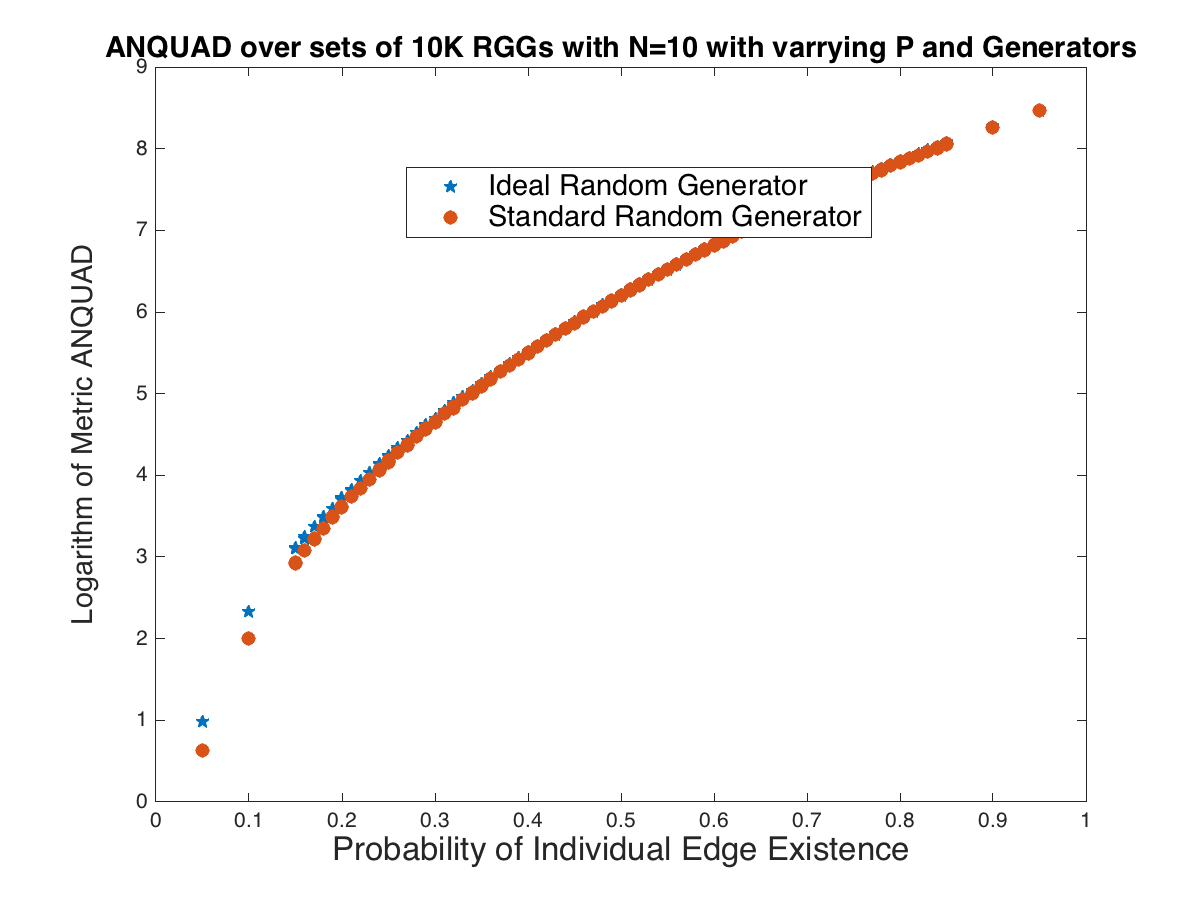
\includegraphics[width=\textwidth]{ANQUAD-10}
\label{fig:anquad10}
\end{figure}

\subsection*{Height Different - ADIAM, ADSMX, ANA, ANCC, ANR, ANTRI, DIAMV, MLNA, NCCV, NUG, PCONN, PDL, PQRA, PQRB, PQRC, SQNR} 
Many of the metrics had the same broad patterns in the way that they changed with respect to $N$ and $p$, but had slightly different heights/inflectuations.
The majority of graph metrics were in this category.
An example shown in figure \ref{fig:sqnr7} shows a metric which rises with duplicates (SQNR) over seven vertices.
Note that though the patterns are the same over the two methodologies, the results are hight separated.

\begin{figure}[h]
\caption{}
\centering
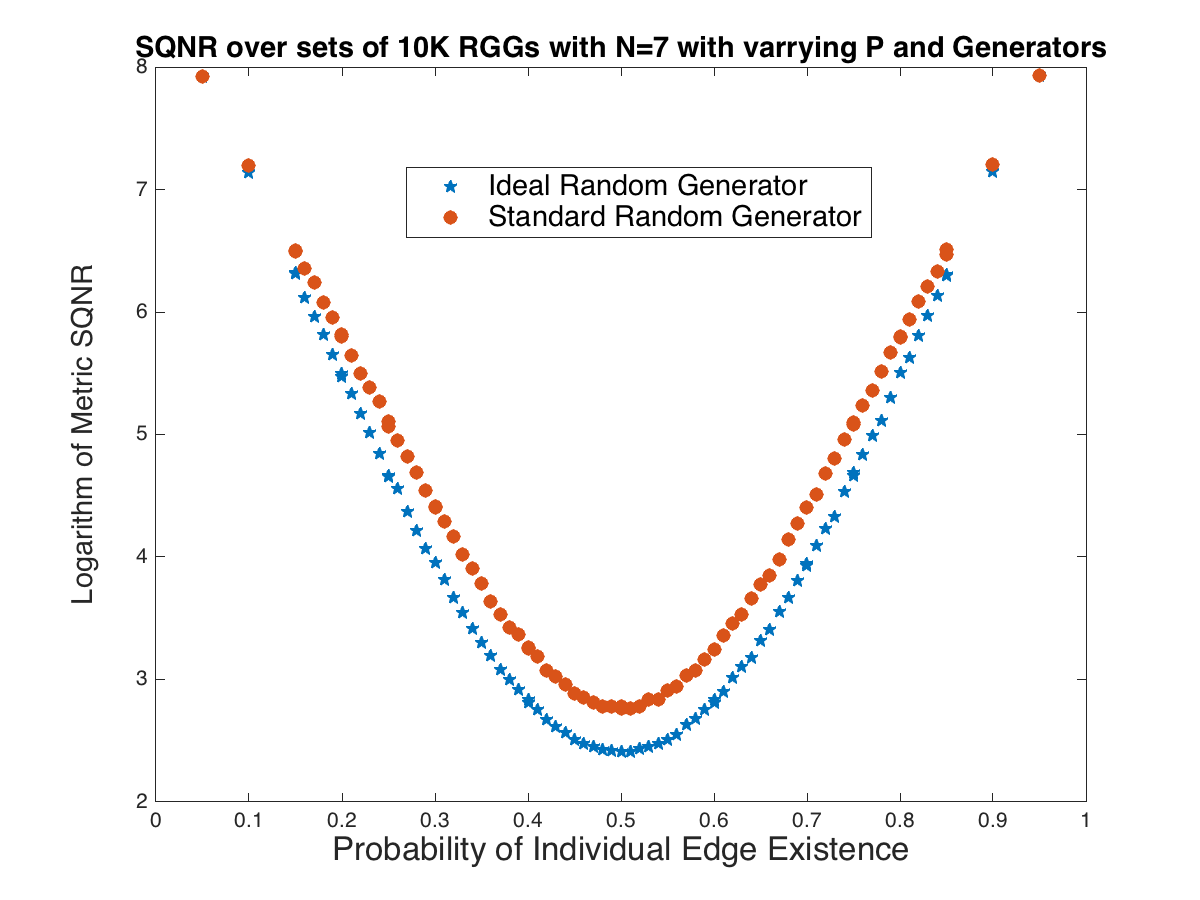
\includegraphics[width=\textwidth]{SQNR-7}
\label{fig:sqnr7}
\end{figure}

\subsection*{Not Enough Data - NCP}
For one metric, there was consistently not enough data to calculate it or any comparison between two random graph generators.
It shouldn't come as a surprise that that metric is NCP, the number of Co-Paths (or Co-Cycles) graphs in the graph set. 
Since there was consistently not enough data to establish a baseline, you will find that most of the time NCP is zeroed out, not by some choice of mine, but because of the way I have set up my scoring mechanism.

\subsection*{Crossover - ADSR, ADSV, NCCV, PTRIL, VLNA}

For five metrics, there was even more of a difference than height alone.
In these graphs, the two curves intersect/cross over so that a metric might be better on one range of $P$ and worse on a different range.
This significantly complicates the way we are able to do optimization to improve upon our graph metric scores. 
With most of the height different variables, clearly we are going to be able to create RGGs which can better mimic a height shift than fundamentally reexamining the nature of the curve.

Two examples are given below, one describes the variance in the diameter of graphs chosen (figure \ref{fig:diamv5}), and the other shows the variation in the logarithm of the number of automorphisms of each graph in the set (\ref{fig:vlna6}).

\begin{figure}[h]
\caption{}
\centering
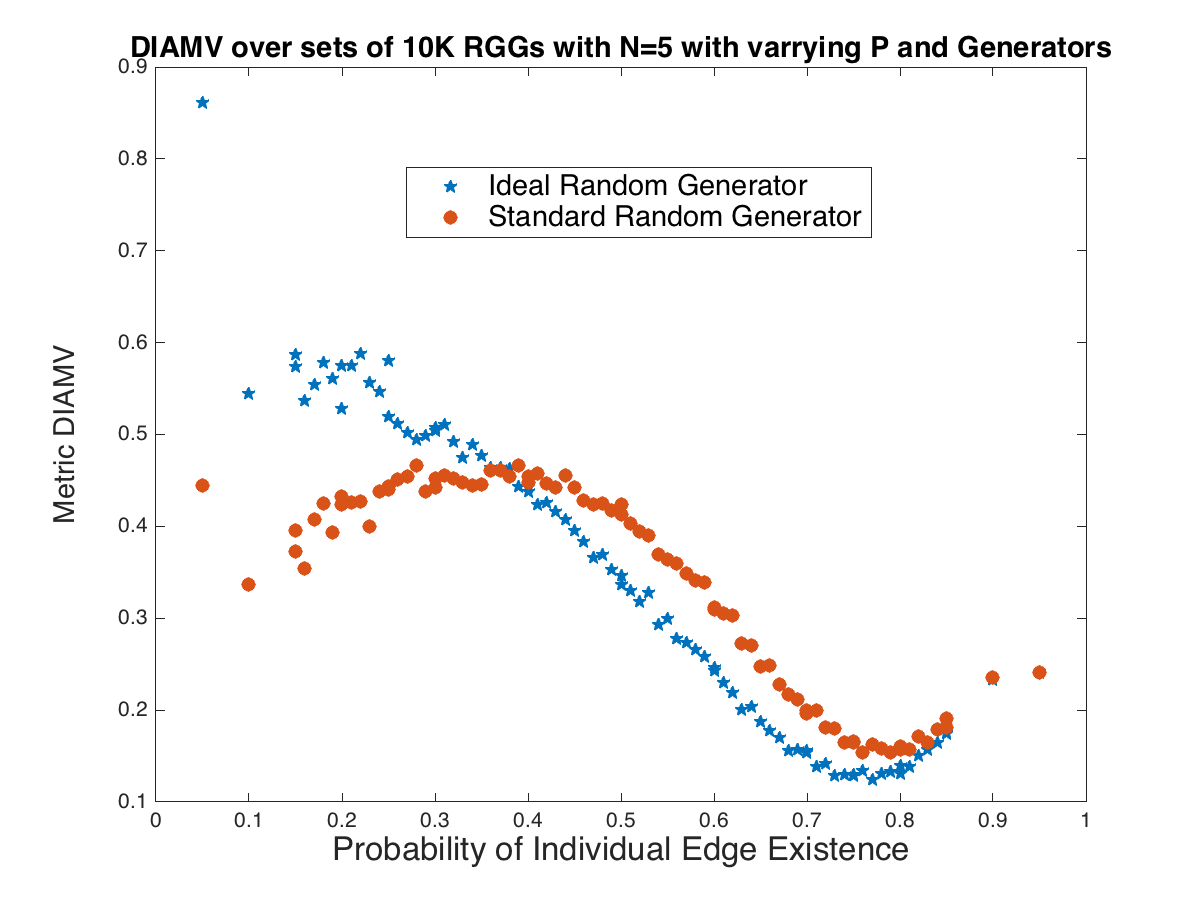
\includegraphics[width=\textwidth]{DIAMV-5}
\label{fig:diamv5}
\end{figure}

\begin{figure}[h]
\caption{}
\centering
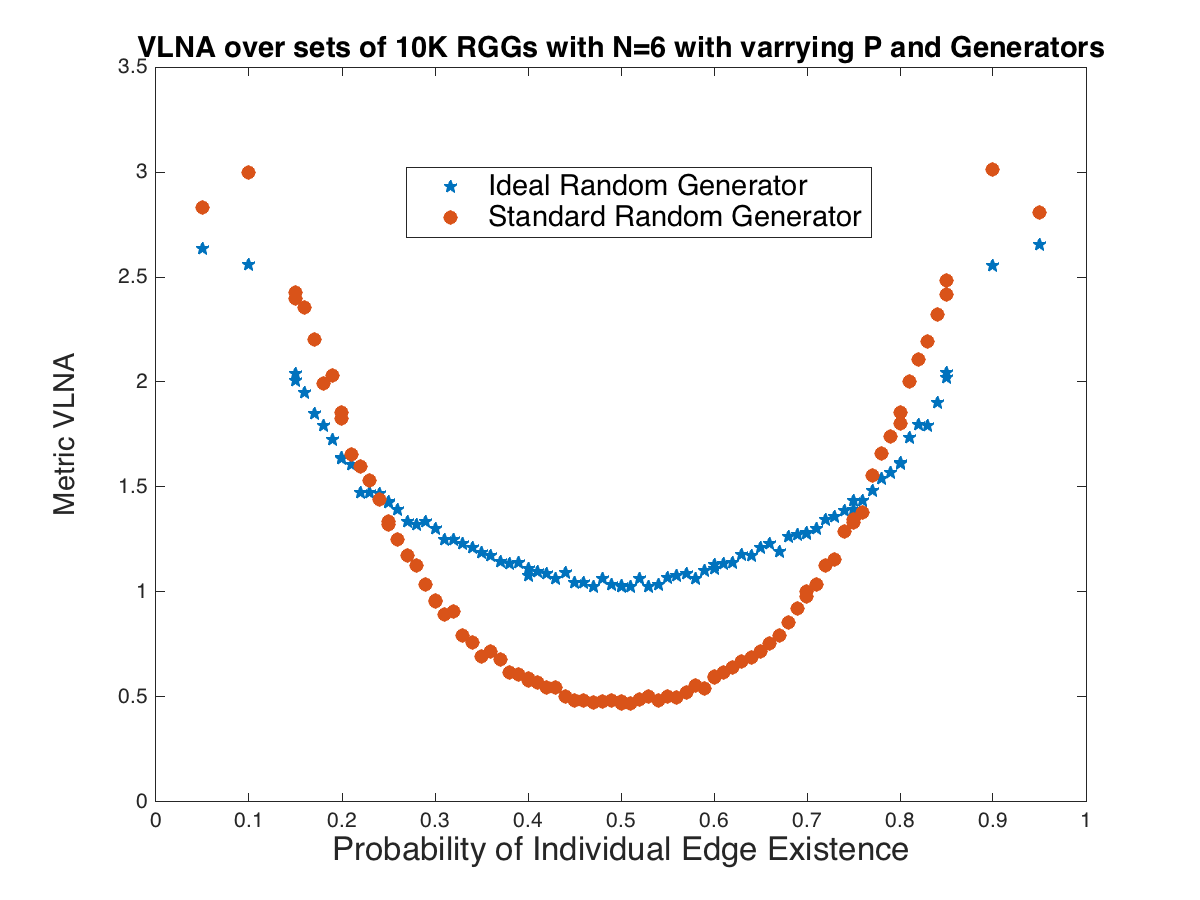
\includegraphics[width=\textwidth]{VLNA-6}
\label{fig:vlna6}
\end{figure}

\subsection*{Shape Different - ALNA, DIAMV, DSMDV, DSMNV, DSMXV, DSVV, MNR, NR}
Finally, many metrics simply displayed different shapes across different ranges of $p$.
Many of these metrics are variance metrics, possibly alluding to the way that graph sets as a whole are either varied or homogenous on each metric.
The two figures displayed show the degree sequence maximum (figure \ref{fig:dsmxv10}), and the average diameter of graphs in the set (figure \ref{fig:adiam9}).
We should remember that these are not trivial differences, and I think that the graphs really speak to that.

\begin{figure}[h]
\caption{}
\centering
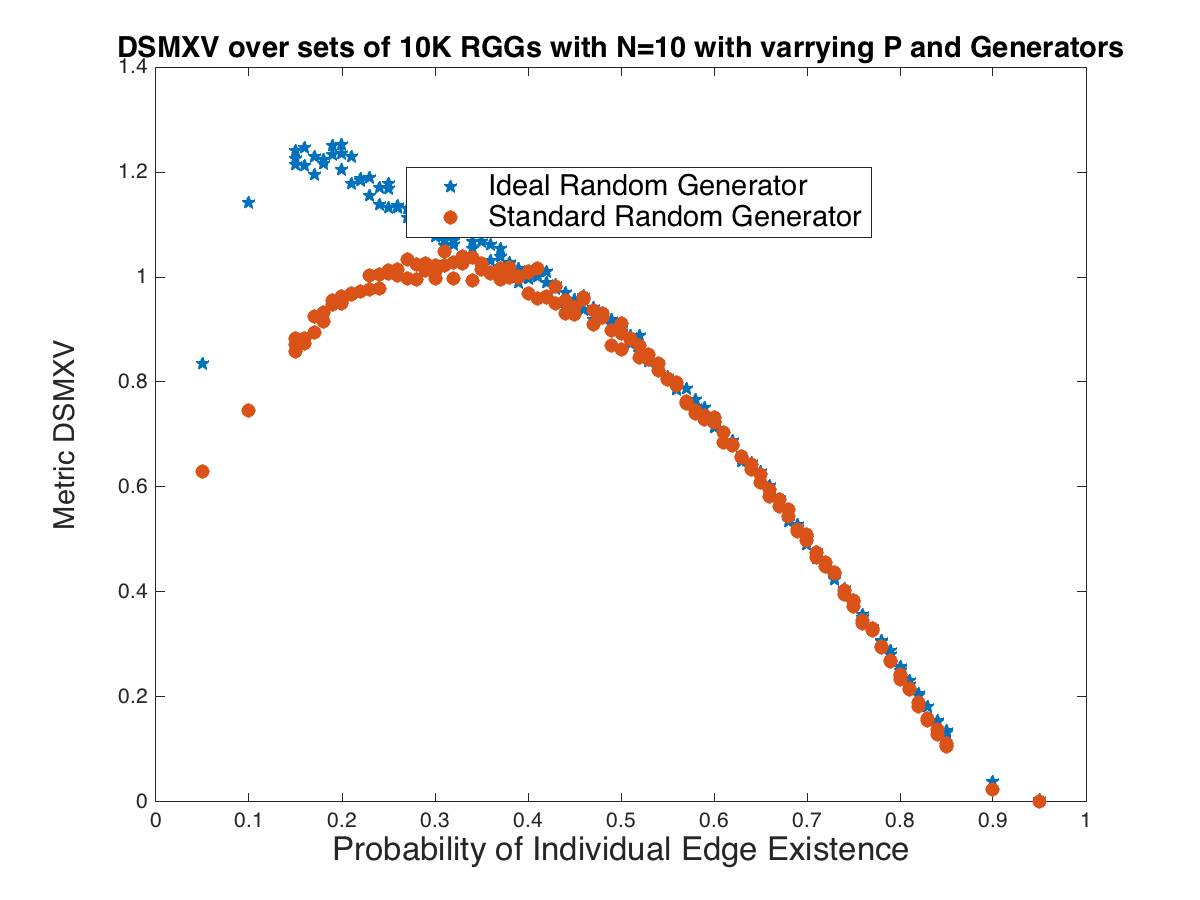
\includegraphics[width=\textwidth]{DSMXV-10}
\label{fig:dsmxv10}
\end{figure}

\begin{figure}[h]
\caption{}
\centering
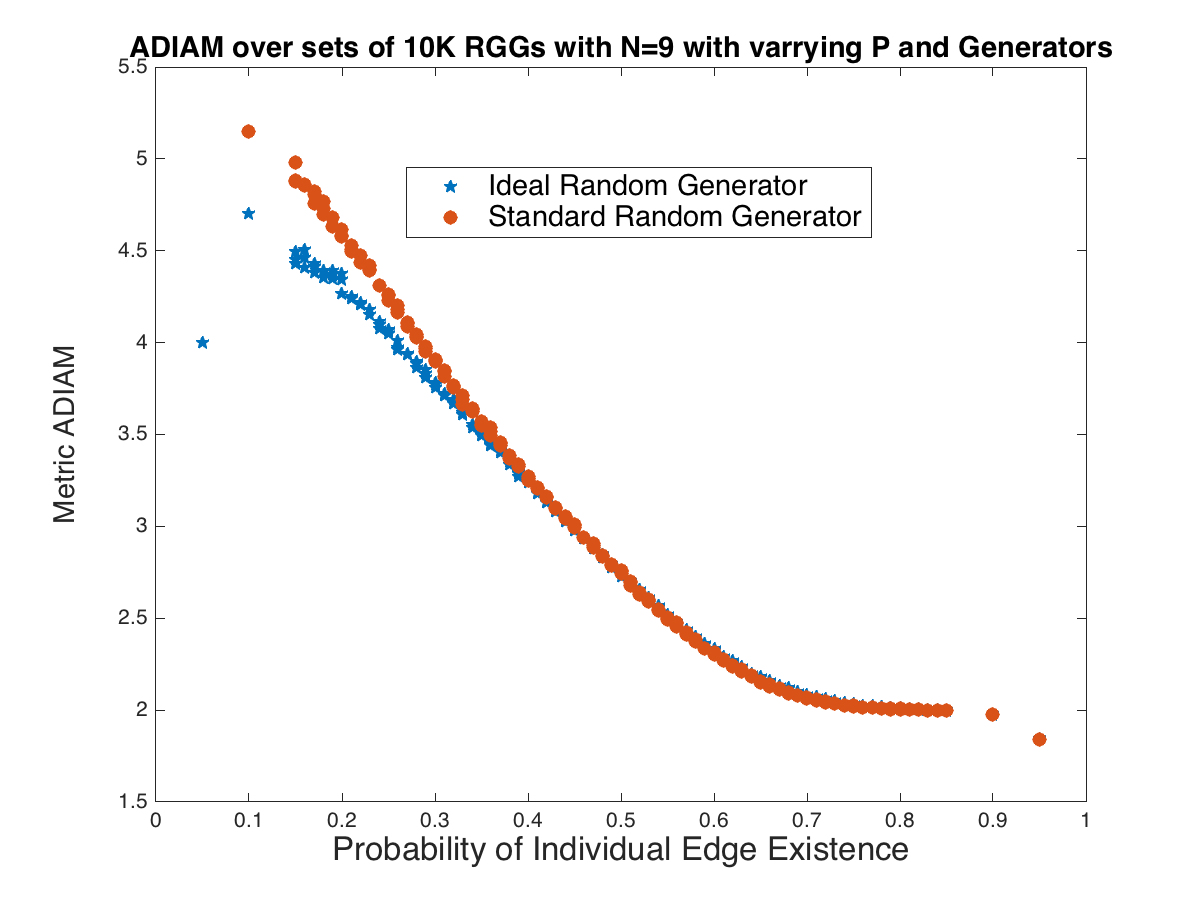
\includegraphics[width=\textwidth]{ADIAM-9}
\label{fig:adiam9}
\end{figure}

\section{Alternative Ideas for Random Graph Modeling and Creation}

Now that we have a mechanism for quantifiably adjudicating the quality of a proposed random graph generator, we are tasked with creating different ideas for random graph generation and evaluating them on this basis.
Discussed below are each of the algorithms that I built for Random Graph Generation and Processing.
They are not presented in any particular order.
Each is prefixed by the string that it is represented as/by throughout the code.

\subsection{MinusOne - A Weighted Automorphic Subgraph Generator}

MinusOne has a simple methodology.
If you are generating a graph with $N$ vertices and with probability of edge creation $p$, start by creating a graph $H$ of size $N+1$ via the gilbert model.
Then, generate all $N+1$ of $H$'s single vertex deleted subgraphs, store each in a set we will call $VD(H)$.
Lets define an automorphic metric $AM$ which is defined by the following formula, finding the QSVSes, and take the product of the factorial of their sizes.
$$AM(g) = \prod_{i \;\in \;QSVSes(g)} |QSVS_i|$$
Finally, over each member of the set $g \in VD(H)$ calculate the automorphic metric, and select that graph with the probability:
$$P(g | H) = \frac{AM(g)}{\sum_{h_i}^{VD(H)} AM(h_i)}$$

\subsection{MinusOneA - Less Automorphic Version of MinusOne}

MinusOneA has a methodology with closely matches that of MinusOne.
The only difference is the automorphic metric function, which is the logarithm of the one proposed above (plus a constant factor).
$$AM(g) = 1 + \log_2 \Big[{\prod_{i \;\in \;QSVSes(g)} |QSVS_i|} \Big]$$

\subsection{MinusOneB - Interspersing Some Gilbert Random Graphs}

MinusOneC has an identical methodology with closely matches that of MinusOne, with one caveat.
With a probability selected based on $p$, the algorithm chooses between picking a graph from a MinusOne distribution and a Gilbert distribution:
\[ MinusOneB(n, p) = \begin{cases} 
      Gilbert(n, p) & \text{if $rand < .5 * (p) * (1-p)$} \\
      MinusOne(n, p) & \text{otherwise} \\
   \end{cases}
\]

\subsection{MinusOneC - Less Automorphic Version of MinusOne}

MinusOneC has a methodology with closely matches that of MinusOne.
The only difference is the automorphic metric function, which is the square root of the one proposed above.
$$AM(g) = \sqrt{\prod_{i \;\in \;QSVSes(g)} |QSVS_i|}$$

\subsection{BuildingA - An Iterative Graph Generator}

Building Algorithms are processes by which edges are added individually to a matrix (given a `probability matrix'), and then a new probability matrix is generated from the current iteration of the formative graph.

\begin{lstlisting}[frame=single]
nEdges = binomalRandom(N, p)
A = zeros(N)
P = (ones(N) - eye(N))/(N*(N-1))
while nEdges > 0:
	A = addEdgeFromProbabilityMatrix(A, p)
	P = generateProbabilityMatrixFromPartialGraph(A)
	nEdges = nEdges - 1
\end{lstlisting}

From this, it is clear that the only place that one can really modify this algorithm is in the generation of the $P$ matrix from the partially generated graph $A$.
BuildingA used a simple algorithm to do this.
It created an edge metric $EM(v_i, v_j)$ to describe the odds of creating an edge between vertices $v_i$ and $v_j$ (here, $DS$ refers to the degree sequence of A as it exists at each iteration):
$$ EM(v_i, v_j, A) = (i - j  \neq 0) * (1 - A[i, j]) * \Big[ 1 + 2 max(DS) - DS[i] - DS[j] \Big] $$
And with the probability of selecting a given edge for creation being:
$$P(\,(v_i, v_j) \,| A) = EM(v_i, v_j, A) / \sum_{x = 1}^{N} \sum_{y = 1}^{N} EM(v_x, v_y, A)$$

\subsection{BuildingB - An Inverse Differential Graph Generator}

The BuildingB random graph generator operates identically to BuildingA, with a change in the individual edge metric $EM_A$:
$$ EM(v_i, v_j, A) = (i - j  \neq 0) * (1 - A[i, j]) * \Big[ 1 + 2 max(DS) + DS[i] + DS[j] \Big] $$

\section{Results}

What I found was that it was consistently harder to beat the benchmarks set out than I had anticipated, however, it was possible.
The detailed score reports are included as an appendix, but the large takeaway was simple:
we are able to construct a random graph generator which mirrors the idealized random graph generator well within the context of these metrics, however, most of our attempts to do so did fail, and were hampered by the strong performance of gilbert random graph generators at larger values of $N$.

In the end, the best algorithm was a composite approach, which was able to score a benchmark of .92 (on a scale of -10 to 10, where 0 represents a gilbert random graph generator). 
The composite approach finds a positive linear combination of results (of different generators) which would approach idealized results, then verifies this linear combination by generating new graphs in their respective proportions and scoring that outcome.
The time constraint of this procedure ran into the final time crunch of this work.
This is the best optimization found, but the large parameter space makes it easy to imagine we could do much better with a more diverse set of algorithms and more time.
This approach (similar to hedge fund management) gives us a good starting place for figuring out how we can better mirror an idealized RGG within a space with limited computational resources (both memory and CPU), via many separate mechansims.
However, I think more work needs to be done to continue figuring out better ways of constructing random graphs which better mirror graphs selected out of the set of graphs, rather than graphs selected out of the set of matrices.
To solve this problem elegantly, we will need to return to algebra.
Approximations of ideal properties will never outperform a theoretically based approach.